%documento de clae
\documentclass[a4paper,12pt]{article}

%paquetes
\usepackage[utf8]{inputenc}
\usepackage[spanish,es-tabla,es-nolayout,es-nodecimaldot]{babel}
\usepackage[total={18cm, 21cm}, top=2cm, left=2cm]{geometry}
\usepackage{amsmath, amssymb, amsfonts, latexsym}
\usepackage{graphicx}
\usepackage[x11names,table]{xcolor}
\usepackage{multicol}
\usepackage{nicefrac}
\usepackage{multirow}
\usepackage{longtable}
\usepackage{booktabs}
\usepackage{url}

%comandos
\title{Escritura de texto matemático}
\author{Alexis Villavicencio}
\date{\today}
\definecolor{db}{RGB}{0,128,128}
\definecolor{dh}{RGB}{128,128,0}

%contenido
\begin{document}
\maketitle
%insercion de tablas
 
 \begin{tabular}{|c|c|c|c|}
  \hline PRIMERA & SEGUNDA & TERCERA & CUARTA \\ \hline
          A      & B       &         & C       \\\cline{1-3}
                 & D       & E       & F        \\ \hline
          G      &         &         & H        \\ \hline
\end{tabular}

 \begin{center}
 \begin{tabular}{ | l | l | l | p{5cm} |}
 % p{5cm}: Quiere decir que me escriba en un parrafo de 5cm
 \hline
 Day & Min Temp & Max Temp & Summary \\ \hline

 Monday & \(11\)C & \(22\)C & A clear day with lots of sunshine.
 However, the strong breeze will bring down the temperatures. \\ \hline
 Tuesday & \(9\)C & \(19\)C & Cloudy with rain, across many northern regions. Clear spells
across most of Scotland and Northern Ireland,
 but rain reaching the far northwest. \\ \hline
 Wednesday & \(10\)C & \(21\)C & Rain will still linger for the morning.
 Conditions will improve by early afternoon and continue
 throughout the evening. \\
 \hline
 \end{tabular}
\end{center}

\begin{center}
\begin{tabular}{|r @{-} l|}
\hline
\(1\) & \(5\) \\ \hline
\(5\) & \(2154\) \\ \hline
\(23\)& \(5\) \\ \hline
\end{tabular} 
\end{center}

\begin{tabular}{|l|l|c|}\hline
 \multicolumn{3}{|c|}{PART\'{I}CULAS AT\'{O}MICAS ELEMENTALES} \\
\hline \hline
\textsf{Part\'{i}cula} & \textsf{Descubridor} & \textsf{A\~{n}o del descubrimiento} \\
\hline
Electr\'{o}n & Joseph J. Thomson* & 1897 \\
\hline
Prot\'{o}n & James Rutherford & 1919 \\
\hline
 Neutr\'{o}n & James Chadwick* & 1932 \\
 \hline
 Positr\'{o}n & Carl D. Anderson* & 1932 \\
 \hline
 \multicolumn{2}{l}{\small *Recibi\'{o} el premio Nobel}
 \end{tabular}

 \begin{tabular}{|c|c|c|}
  \hline \multicolumn{3}{|c|}{Team sheet} \\ \hline
  \hline \multirow{3}{*}{Pivots}&36&Gasol\\ \
  &23& O\'{}Neal\\ 
  &45& Howard \\ \hline
 \end{tabular}
 \\
 \(1.2\)
 \begin{center}
\begin{tabular}{|>{\columncolor{db!20}} c | c | >{\color{magenta}} c |}
\hline
\rowcolor{db}
\hline
\color{yellow!30!white} \textbf{Temperatura} &
\color{yellow!30!white} \textbf{Tiempo} &
\color{yellow!30!white} \textbf{Total} \\ \hline
1 & \(245 \pm 5.5\) & 3 \\ \hline
2 & \(260 \pm 5.5\) & \cellcolor{white!70!dh}\color{dh}{8} \\ \hline % para pintar una sola celda
 3 & \(275 \pm 5.5\) & 8 \\ \hline
 4 & \(287 \pm 5.5\) & 8 \\ \hline
 \end{tabular}
 \end{center}
 
 \begin{longtable}{lll}
\caption{Lista de Estudiantes} \\
\toprule
\textbf{Nombre} & \textbf{Carrera} & \textbf{Correo electrónico} \\
\midrule
\endfirsthead
%
\multicolumn{3}{l}{\footnotesize Viene de la página anterior} \\
\toprule
\textbf{Nombre} & \textbf{Carrera} & \textbf{Correo Electrónico} \\ \midrule
\endhead
\bottomrule \multicolumn{3}{r}{\footnotesize Continua en la siguiente página}
\endfoot
\bottomrule
\endlastfoot
%
Milton Torres & Matemática & \url{mate6666oz@hotmail.com}\\
Milton Torres & Matemática & \url{mate6666oz@hotmail.com}\\
Milton Torres & Matemática & \url{mate6666oz@hotmail.com}\\
Milton Torres & Matemática & \url{mate6666oz@hotmail.com}\\
Milton Torres & Matemática & \url{mate6666oz@hotmail.com}\\
Milton Torres & Matemática & \url{mate6666oz@hotmail.com}\\
Milton Torres & Matemática & \url{mate6666oz@hotmail.com}\\
Milton Torres & Matemática & \url{mate6666oz@hotmail.com}\\
Milton Torres & Matemática & \url{mate6666oz@hotmail.com}\\

\end{longtable}

%insercion de graficos
\begin{center}
 
\includegraphics[scale=2]{papa}
\end{center}

\begin{center}
 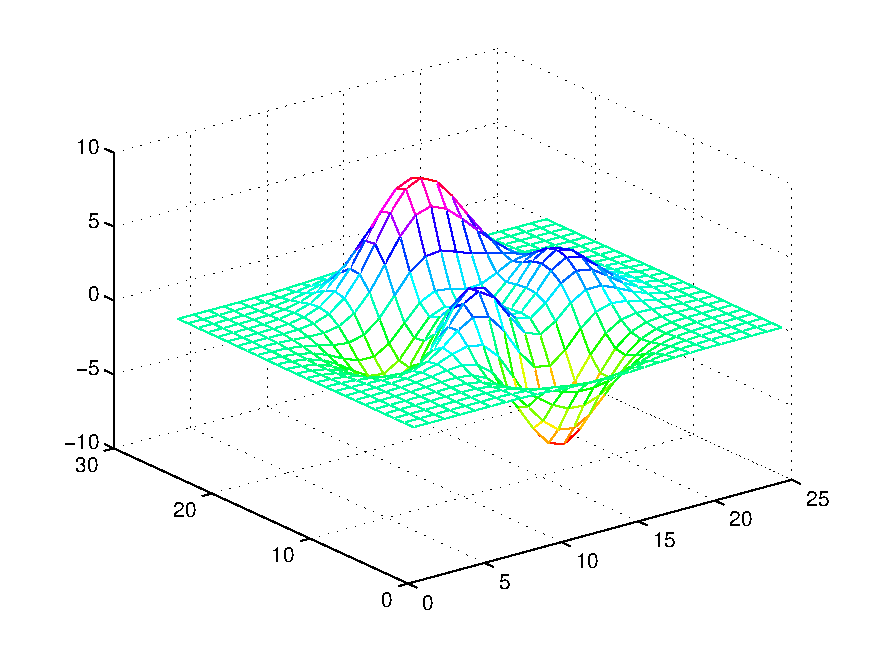
\includegraphics[scale=0.5,width=15cm,angle=65]{figura1.pdf}
\end{center}
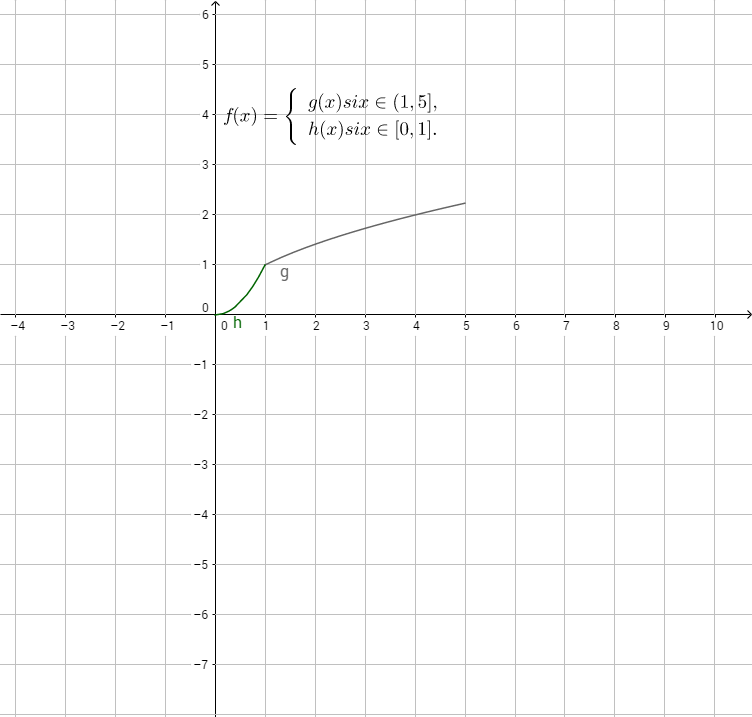
\includegraphics[scale=0.7]{figura2}
\end{document}
